%!TeX program=pdflatex
%!TeX encoding=utf8
%!TeX spellcheck = en_GB
%!TeX root = ../../messageVortex.tex

\part{Results}
To verify the hypothesis made in this paper, and to analyse properties of the protocol in a real world scenario a library was implemented in Java which was capable of handling all message packets and the routing stack as a whole. The following paragraphs describe the protocol developed in general as a generic approach. Appendix \ref{app:asnone} gives the full ASN.1 representation of the protocol. 

It is important to notice that ASN.1 has no mean to express encrypted structures. Due to this fact we defined all encrypted fields as \verb|OCTET STRING|. The protocol offers according to the ASN.1 the possibility to store onionized information in an unencrypted form. This is meant for debuing purposes. At no point this should be used in a production environment.

The protocol described in the next chapter is independent from routing. At the moment capabilities include SMTP and XMPP. The protocol may be extended by adding new transport layer capabilities and their addressing schemes.

\chapter{MessageVortex - Transport Independent Messaging anonymous to \nth{3} Parties}
This approach is different from all approaches discussed previously. Unlike them we put complete distrust into the infrastructure being used. Furthermore we do not rely on a custom server infrastructure in the internet. Instead we take advantage of the availability of internet connected devices such as internet connected mobile phones, tablets, or even commonly available SoC such as RaspberryPi or similar. It is still very hard to maintain a server in the internet and considering the vastly growing amount of automated attack carried out against internet connected servers it is not advisable or realistic to assume that a future user of this system owns either a server or connects to a service which is offering explicitly anonymizing services. These infrastructures would be suspectible to monitoring or even banning. Instead we take a different approach.

We use common messaging protocols as transport layers and connect to them using the respective client protocols. The actual mixes are operated by the users on their ``always connected'' devices. It goes without saying that such a system is far less reliable than a traditionally run server as this hardware is typically cheap and normally connected to the internet using a bandwidth shared media.

The basic idea is that a client generates all traffic (including decoy or dummy traffic) by itself. It defines the routes a message takes through the mixes and decides which targets are receiving dummy traffic at the same time. In such a system even when possessing all the nodes routing the traffic (without the endpoints) an anonymity set of $k$ (whereas the size of $k$ is defined by the sender) is guaranteed.

As decoy traffic is generated with the same operations as the true content is split it is impossible for an adverser running a node to determine wether he is generating noise or actually processing the true message.

\fxfatal{add a lot more text here}
\begin{figure}[h]
	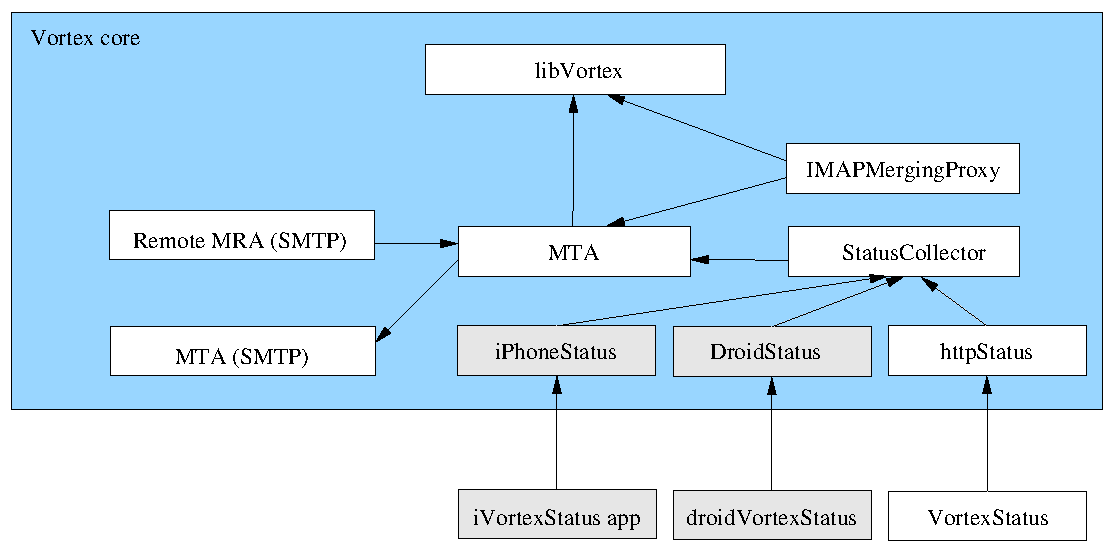
\includegraphics[width=\columnwidth]{inc/VortexModules.pdf}
	\caption{Overview of the Vortex modules}
	\label{fig:vortexModules}
\end{figure}

\section{Protocol Description}
\section{Accounting}
\section{Message Flows}

\section{Considerations for Building Messages}
In a worst case scenario we assume that an adverser is controlling most of the network utilized for anonymisation. While this is not nessessarily a problem (as pointed out earlier) it allows an adverser to track a message while agents are being used under his control. So for simplicity and as a worst case assumption we always assume that an adverser has perfect knowledge of an associated message flow. This is however a worst case scenario. One missing agent disconnects the whole chain and as messages are not traceable in size.

\subsection{Ephemeral identities}
\fxfatal{expiring ephemeral identities shold not only be replaced after their expiration but anytime during the livetime}
\subsection{Timing of messages}
\fxfatal{add content here}

\subsection{Building Diagnostic Paths}
\fxfatal{add content here}

\subsubsection{Implicit Diagnostic}
\fxfatal{Add comments about messages splitting and returning to sender}

\subsubsection{Automatic Explicit Diagnostic}
\fxfatal{Add comments about error and diagnosis messages officially spliting of messages}

\subsubsection{On-Demand Explicit Diagnostic}
\fxfatal{Add comments about normal, error, and diagnosis messages beeing picked up by a routing block}

\section{Considerations for Routing Messages}
\subsection{Time of sending}
Messages should always be sent timewise nearby other messages. This means that the best moment for sending a message in a ready queue is at a time when sending of other messages is due. However no optimisation should be done to send as many messages as possible at the same time. this would lead to a forseeable behaviour of the routing layer and thus to misusable behaviour.



\section{Real World Considerations}
This approach is heavily dependent of the transport protocol and builds on top a new obfuscating/routing layer. For this system to become a real peer-to-peer approach some additional quirks are required. A message-Vortex-Account needs always an active routing handler. This routing handler may be introduced by new server capabilities or by having a device handling the routing from the client side. For this reason we built a RaspberryPi appliance capable of connecting to one (or more) accounts fetching incomming mails, analysing them and reroute them if necessary. Although the system is designed to be run on a RaspberryPi the software might be installed to any Java capable client. The RaspberryPi is just an affordable lightweight device which offers all required capabilities.

\chapter{Security Analysis}
\fxfatal{add content here}

\chapter{Additional Considerations}
\section{Man in the Middle Attacks to Conversations}
\fxfatal{add content here}

\section{Identification of participating account}
\fxfatal{add content here}

\subsection{Identification by Query}
\fxfatal{add content here}

\subsection{Identification by Traffic Type}
\fxfatal{add content here}

\subsection{Identification by Bandwidth}
\fxfatal{add content here}

\subsection{Identification by Behavioural analysis}
\fxfatal{add content here}

\section{Storage of Messages and queues}
The storage of messages sent though MessageVortex should be handled with great care. It seems on the first sight a good idea to merge all messages in a globally available storage such as the mail account of the receiving entity. However -- In doing so we would discover the message content to the providing party of a mail account. Since we handled the message with great care and tremendous costs up until this point it would be careless doing so. 

Storing them in a localized and receiving entity controlled storage is definitely a good idea but leaves security considerations like a backup possibly to an end user. This might be better but in effect a questionable decision. There is however a third option. By leaving the message unhandled on the last entity of the MessageVortex chain we may safely backup the data without disclosing the message content. Merging the content then dynamically through a specialized proxy would allow the user tu have a unified view on his without compromising the security.

\fxfatal{implemented in prototype?}

\section{Economy of transfer}
\fxfatal{Write something about wasting bandwidth}